\documentclass[12pt,aspectratio=169]{beamer}

\usetheme{metropolis}

\definecolor{mDarkBrown}{HTML}{FF5722}
\definecolor{mDarkTeal}{HTML}{263238}
\definecolor{mLightBrown}{HTML}{FF5722}

\usepackage{booktabs}
\usepackage{graphicx}
\usepackage{hyphenat}
\usepackage{multirow}
\usepackage{nicefrac}
\usepackage[normalem]{ulem}

\usepackage[weather]{ifsym}

\usepackage{pifont}
\newcommand{\cmark}{\ding{51}}
\newcommand{\xmark}{\ding{55}}

\usepackage{minted}
\usemintedstyle{tango}
\newminted[bash]{bash}{%
    autogobble,
    bgcolor=mDarkTeal!10,
    linenos
}
\newminted[py3]{python}{%
    python3,
    autogobble,
    bgcolor=mDarkTeal!10,
    linenos
}
\newminted[sql]{sql}{%
    autogobble,
    bgcolor=mDarkTeal!10,
    linenos
}

\usepackage{polyglossia}
\setdefaultlanguage[variant=british]{english}
\usepackage[english=british]{csquotes}

\defaultfontfeatures{Ligatures=TeX}
\setmainfont{Lucida Sans OT}
\setsansfont[Scale=MatchLowercase]{Lucida Sans OT}
\setmonofont[Scale=MatchLowercase]{Lucida Console DK}

\usepackage{mathspec}
\setmathsfont(Digits,Latin,Greek)[Numbers={Lining,Proportional}]{Lucida Bright Math OT}

\newcommand{\mat}[1]{\ensuremath{\mathbf{#1}}}

\newcommand{\R}{\ensuremath{\mathbb{R}}}

\newcommand{\E}[1]{\ensuremath{\mathbb{E}\!\left[ #1 \right]}}
\newcommand{\V}[1]{\ensuremath{\mathbb{V}\!\left[ #1 \right]}}
\newcommand{\Prob}[1]{\ensuremath{\Pr\!\left( #1 \right)}}
\newcommand{\Normal}[2]{\ensuremath{\mathcal{N}\!\left( #1, #2 \right)}}
\newcommand{\simiid}{\ensuremath{\overset{\text{\tiny i.i.d.}}{\sim}}}

\DeclareMathOperator{\logit}{logit}

\author{Gianluca Campanella}
\date{}



\title{Version control with Git and GitHub}

\begin{document}

\maketitle

\begin{frame}{Contents}
    \tableofcontents[hideallsubsections]
\end{frame}

\section{Version control systems}

\begin{frame}{What is version control?}
    \only<1>{%
        \begin{center}
            
\includegraphics[height=0.8\textheight]{figures/final} \\
            {\scriptsize%
             From \textit{PHDComics.com}}
        \end{center}}
    \only<2>{%
        A version control system (VCS) allows you to\ldots\vspace{-1ex}
        \begin{itemize}
            \item \alert{Records changes} to files
            \item \alert{Revert back} to a previous state
            \item \alert{Compare changes} over time and contributors
        \end{itemize}
        \vfill
        \begin{block}{Types}
            \begin{itemize}
                \item \alert{Centralised} VCS: CVS and Subversion (SVN)
                \item \alert{Distributed} VCS: Git and Mercurial
            \end{itemize}
        \end{block}}
    \only<3>{%
        \vfill
        \begin{columns}
            \begin{column}{0.5\textwidth}
                \centering
                \textbf{Centralised VCS} \\[\bigskipamount]
                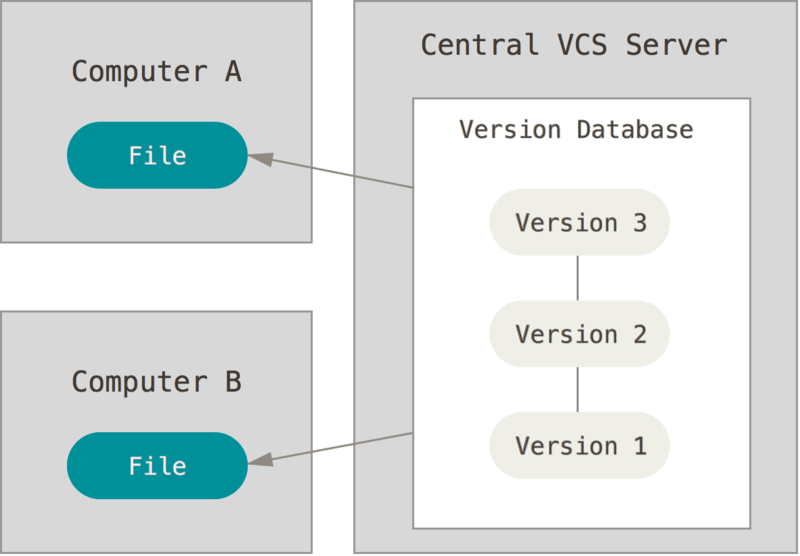
\includegraphics[height=0.6\textheight]{figures/centralized_vcs} \\
            \end{column}
            \begin{column}{0.5\textwidth}
                \centering
                \textbf{Distributed VCS} \\[\bigskipamount]
                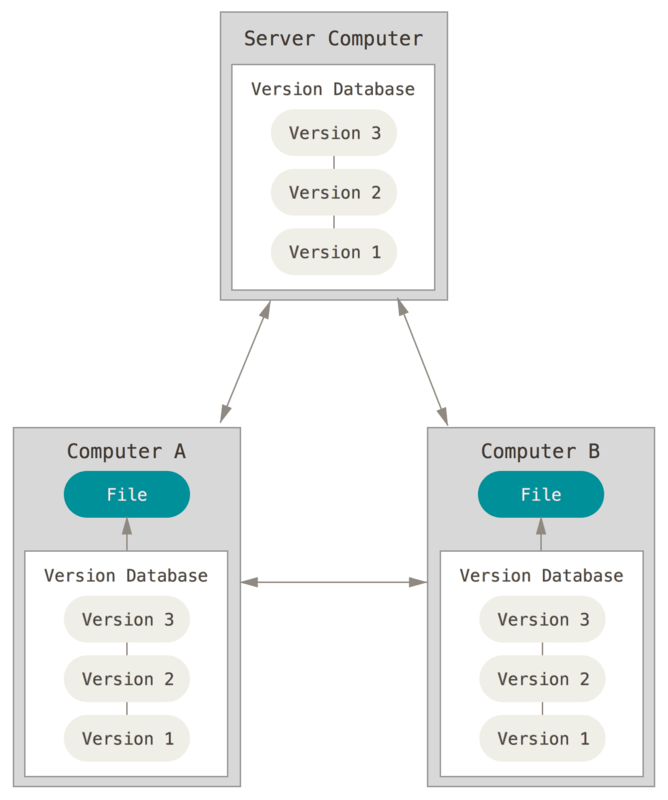
\includegraphics[height=0.6\textheight]{figures/distributed_vcs} \\
            \end{column}
        \end{columns}
        \vfill
        \begin{center}
            {\scriptsize%
             From \textit{Pro Git}}
            \vspace{-3em}
        \end{center}}
\end{frame}

\begin{frame}{What are Git and GitHub?}
    \begin{columns}[t]
        \begin{column}{0.5\textwidth}
            \begin{center}
                \textbf{Git}
            \end{center}
            \begin{itemize}
                \item Distributed VCS
                \item Free and open\hyp{}source
                \item Originally developed by \\ Linus Torvalds
                \item Repositories, branches, commits, merges, \ldots
            \end{itemize}
        \end{column}
        \begin{column}{0.5\textwidth}
            \begin{center}
                \textbf{GitHub}
            \end{center}
            \begin{itemize}
                \item Company
                \item Provides Git hosting
                \item Web interface
                \item Issue tracker, pull requests, wikis, \ldots
            \end{itemize}
        \end{column}
    \end{columns}
\end{frame}

\section{Git}

\begin{frame}{Some terminology}
    \vspace{0.5em}
    \begin{block}{Repository (or `repo')}
        A set of tracked files
    \end{block}
    \vfill
    \begin{block}{Commit}
        Record changes to the repository (create a `snapshot')
    \end{block}
    \vfill
    \begin{block}{Push/pull}
        Update remote/local repository using local/remote repository
    \end{block}
    \vfill
    \begin{block}{Branch (fork)}
        Different version of a repository (stored in a different account)
    \end{block}
    \vfill
    \begin{block}{Merge}
        Join two development histories (branches/forks) together
    \end{block}
\end{frame}

\begin{frame}{Git workflow}
    \begin{center}
        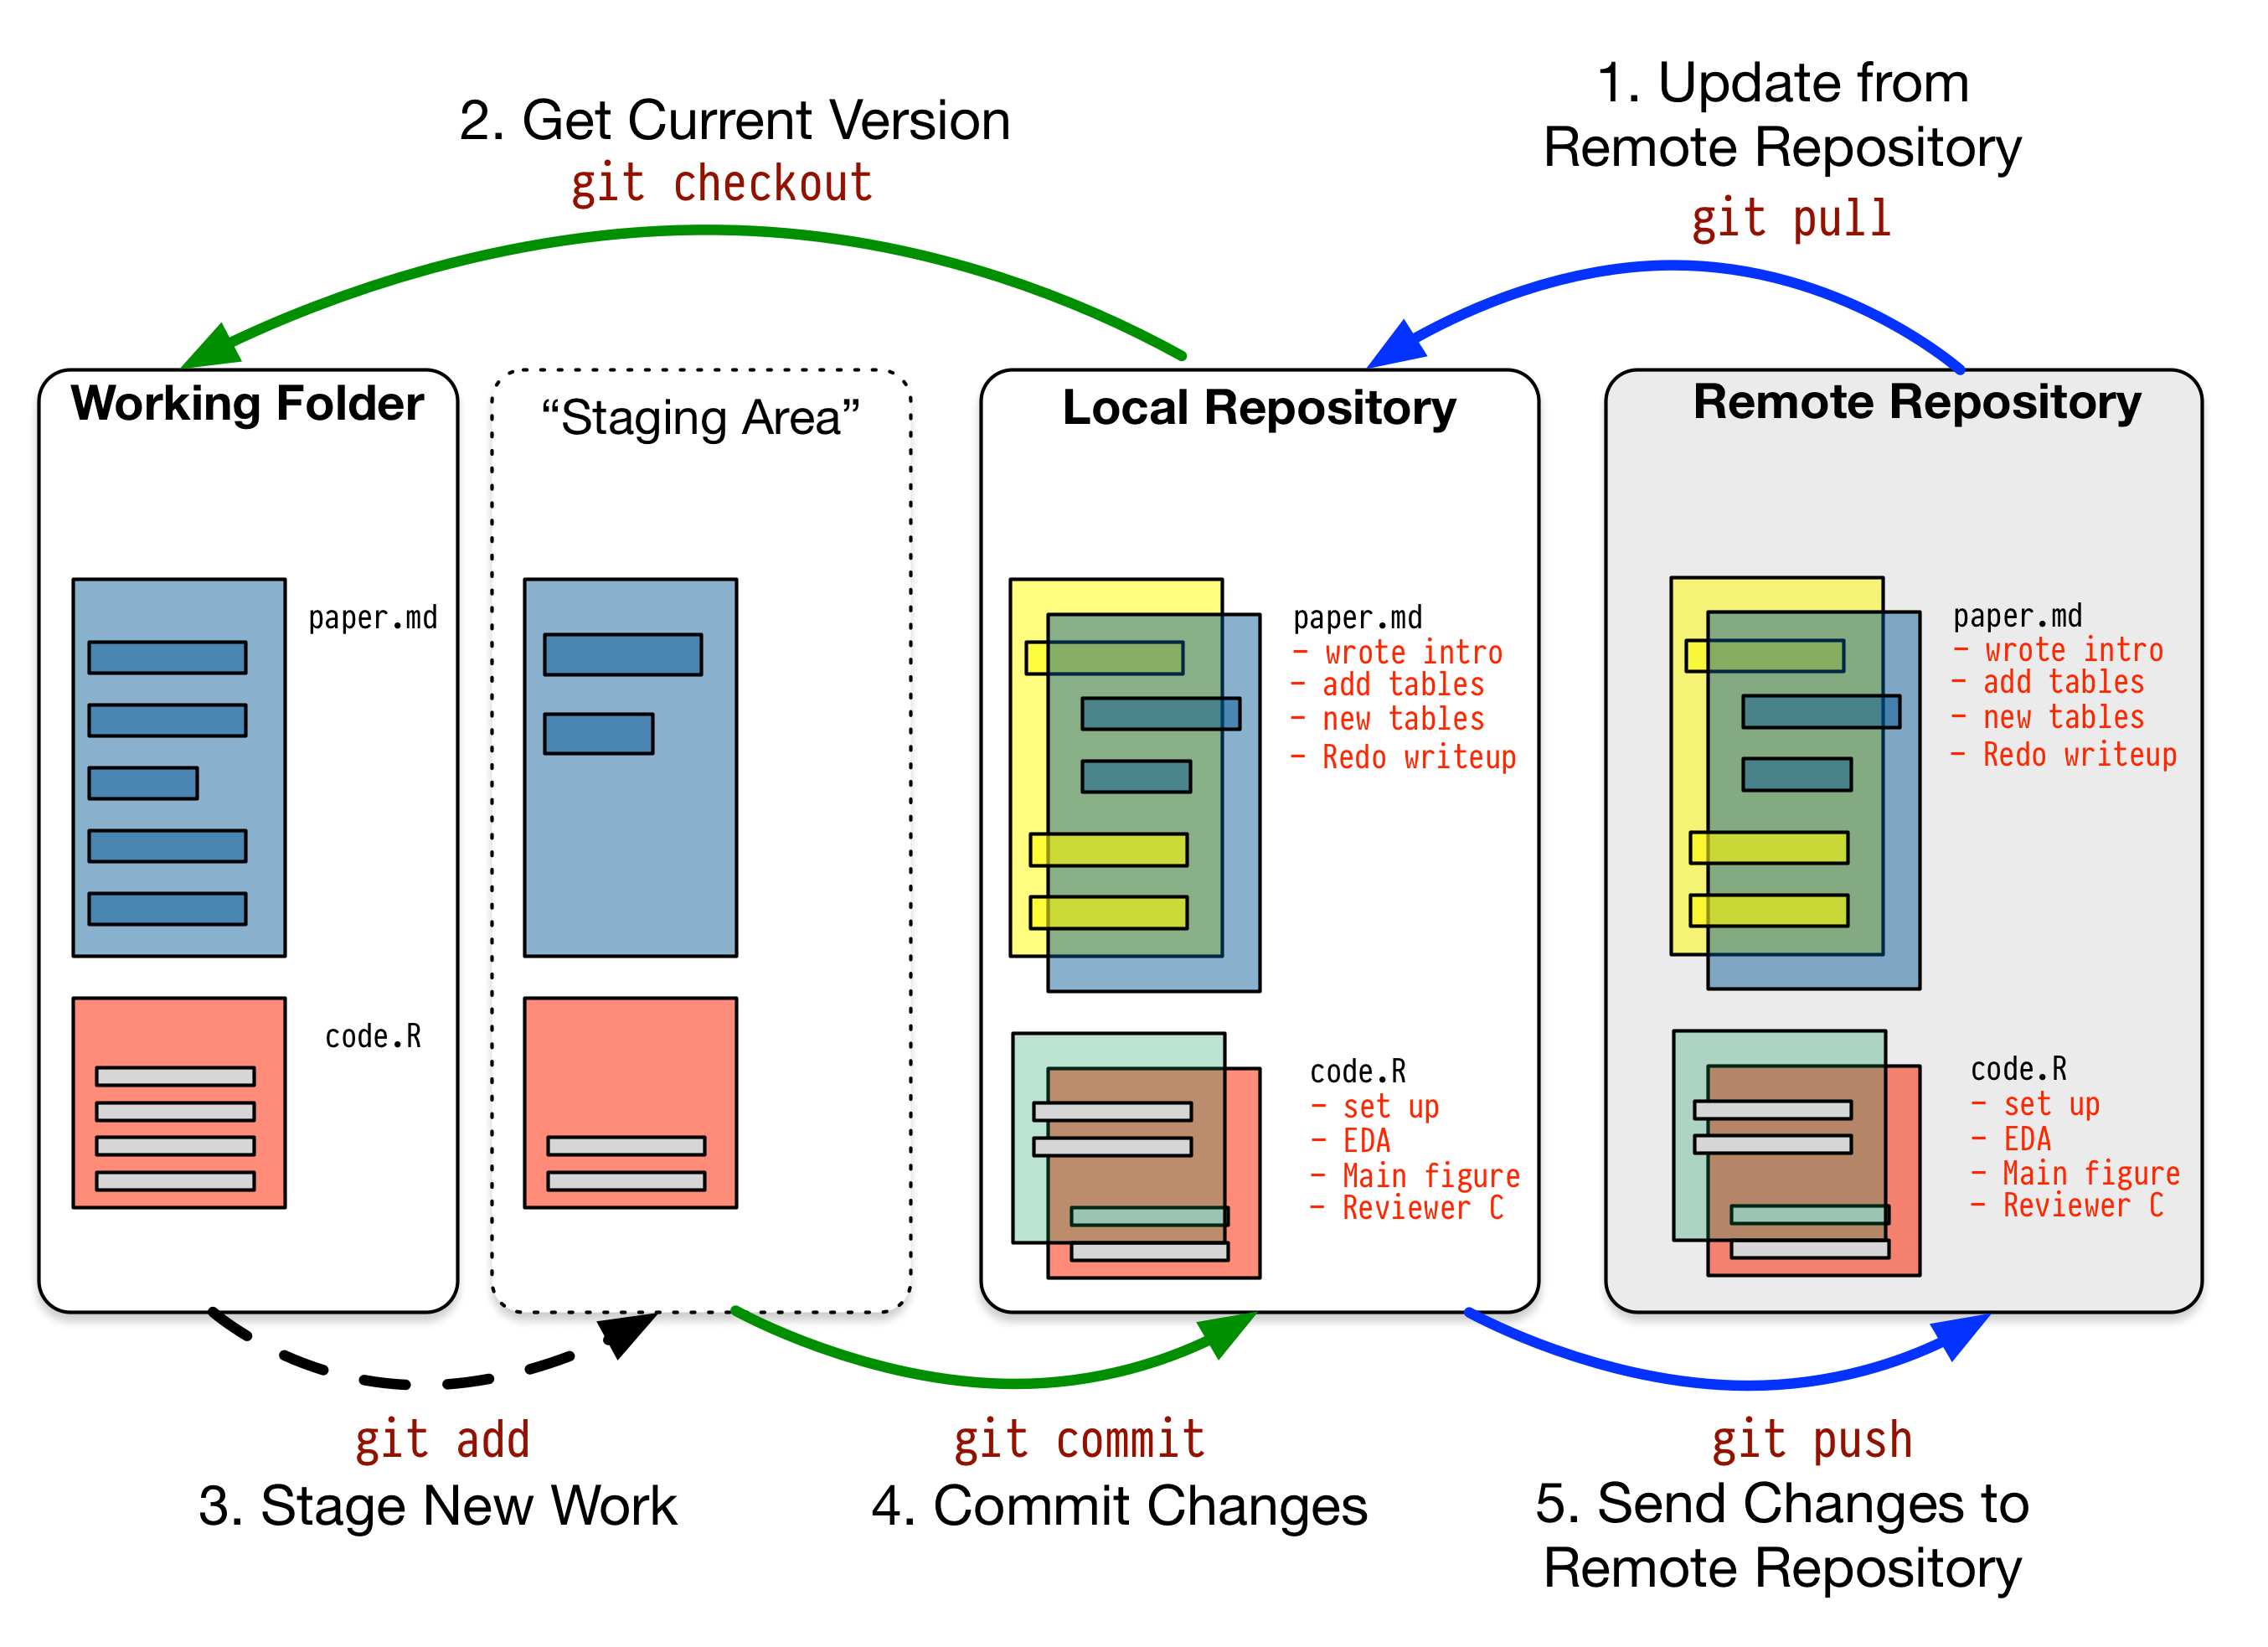
\includegraphics[height=0.8\textheight]{figures/git_workflow} \\
        {\scriptsize%
         From \textit{The Plain Person's Guide to Plain Text Social Science}}
    \end{center}
\end{frame}

\begin{frame}{Commit messages}
    \begin{center}
        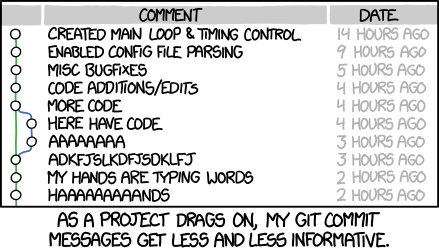
\includegraphics[width=0.5\textwidth]{figures/git_commit} \\[\bigskipamount]
        {\scriptsize%
         From \textit{xkcd.com}}
    \end{center}
\end{frame}

\section{GitHub}

\begin{frame}{Making your repository available on GitHub}
    \begin{itemize}
        \setlength{\itemsep}{\bigskipamount}
        \item Not needed if you only want to keep track of your code locally
        \item Good idea for \alert{collaborative work}, or if you want to\ldots
              \begin{itemize}
                  \item Showcase to the world what you're working on
                  \item Share projects that might be of interest to others
                  \item Contribute to open\hyp{}source software
              \end{itemize}
        \item Other Git hosting options exist (e.g.\ GitLab)
    \end{itemize}
\end{frame}

\begin{frame}[fragile]{Pushing, pulling, and cloning}
    \vspace{1em}
    \begin{block}{Push}
        \begin{bash}
            git push <remote> <local_branch>
            git push origin master
        \end{bash}
    \end{block}
    \vspace{-0.5em}
    \begin{block}{Pull}
        \begin{bash}
            git pull <remote>
            git pull origin
        \end{bash}
    \end{block}
    \vspace{-0.5em}
    \begin{block}{Clone}
        \begin{bash}
            git clone https://github.com/<username>/<repository>
        \end{bash}
    \end{block}
\end{frame}

\end{document}

